\chapter{二元液–蒸气图与蒸馏}\label{ch:b2:liquid-vapour-diagrams}

铜制蒸馏釜可将酒精含量仅百分之几的葡萄酒，
变为浓度高出许多倍的烈酒；炼油塔则把原油切割成从气体
到重质燃料的各个馏分。两者都依赖同一事实：沸腾混合物上方的蒸气
中易挥发组分的含量高于液体。反复进行
蒸发与液化，只要次数足够多，分离便可达到所需的
任意锐度——唯一的例外是：无论蒸馏塔多高，
乙醇的质量分数都无法超过约 95\%。本章给出
描述两种液体混合物如何沸腾的相图，并利用它们
设计蒸馏塔，判断分离必须止于何处。

\begin{recall}
\Cref{ch:b2:chemical-potential}：化学势、拉乌尔定律，以及
理想混合物、活度系数及对拉乌尔定律的偏离，
吉布斯–杜安关系。\Cref{ch:b2:equilibrium-shifts}：自由度。
本科一年级分册讲实验技术：简单蒸馏，互溶与
不互溶液体。第 1 册讲：蒸馏与水蒸气蒸馏。
\end{recall}

\begin{omfigure}
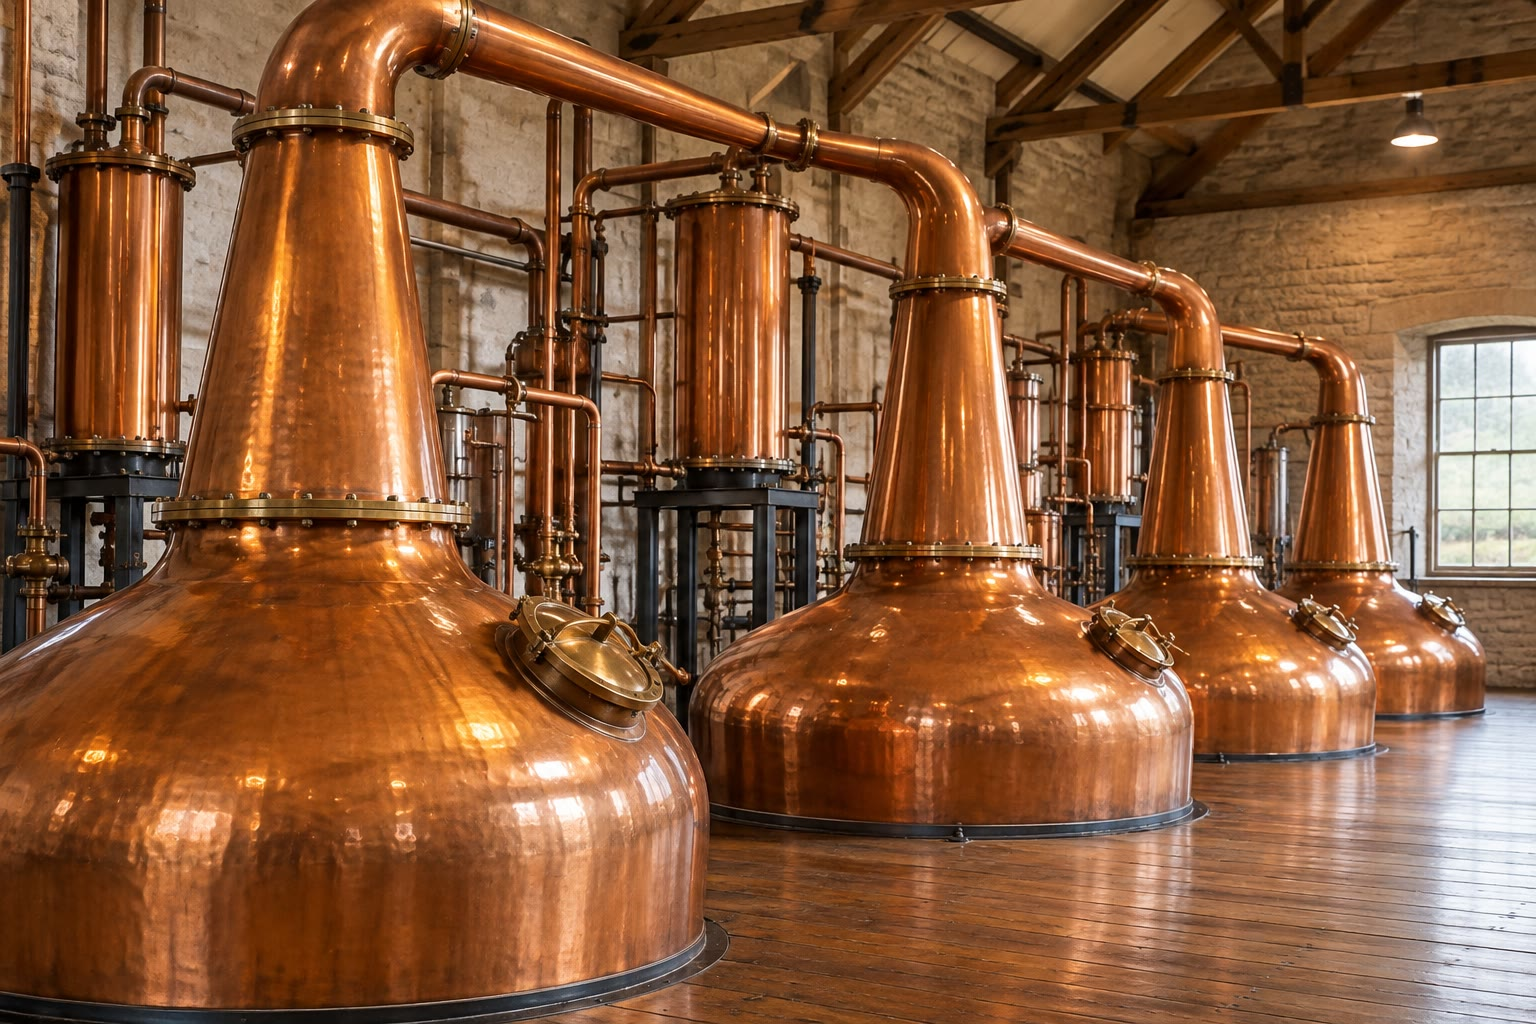
\includegraphics[width=0.62\linewidth]{images/book3/ai/b2-07-pot-stills.jpg}

{\small 酒厂中的铜制罐式蒸馏釜。每次装入的发酵醪
被加热煮沸，其蒸气冷却凝结：第一次馏出液的乙醇含量
为发酵醪的数倍，再次蒸馏可使其进一步浓缩。}
\end{omfigure}

\section{理想混合物}

本章将两种液体编号为 1（较易挥发、沸点较低者）和 2，
其中 $x$ 为液相中组分 1 的摩尔分数，$y$ 为其
气相中的摩尔分数，该气相视为理想气体。

\begin{definition}[二元相图]\label{def:b2:liquid-vapour-diagrams:binary-diagram}
\emph{二元相图}\index{二元相图}表示，对于两组分混合物，
哪些相存在、各相的组成如何，作为
总组成与另一变量的函数。
\emph{等压相图}\index{等压相图}画在（组成，温度）平面上，压强固定；
而\emph{等温相图}\index{等温相图}
画在（组成，压强）平面上，
温度固定。
\end{definition}

\begin{definition}[泡点线与露点线]\label{def:b2:liquid-vapour-diagrams:bubble-dew}
在液–蒸气相图上，\emph{泡点线}\index{泡点线}给出与蒸气平衡的液相组成，
而\emph{露点线}\index{露点线}给出与液相平衡的蒸气组成。
对于给定组成、压强固定的混合物，
\emph{泡点}\index{泡点}是加热时
出现第一个气泡的温度，
\emph{露点}\index{露点}是
冷却蒸气时出现第一滴液体的温度。
\end{definition}

\begin{proposition}[理想曲线]\label{prop:b2:liquid-vapour-diagrams:ideal-curves}
对于温度为 $T$ 的理想混合物，设 $p_1^*$ 与 $p_2^*$ 为
两纯液体的蒸气压，则等温相图的泡点线是
直线 $p = p_2^* + x(p_1^* - p_2^*)$，
露点线为双曲线
\[
  p = \frac{1}{y/p_1^* + (1 - y)/p_2^*} .
\]
\end{proposition}

\begin{proof}
由拉乌尔定律得分压 $p_1 = xp_1^*$ 与 $p_2 = (1 -
x)p_2^*$，二者之和即总压，关于 $x$ 呈线性。在气相中，
有 $y = p_1/p$，故 $x = yp/p_1^*$，$1 - x = (1 - y)p/p_2^*$；相加得
$1 = p\,[y/p_1^* + (1 - y)/p_2^*]$。
\end{proof}

\begin{proposition}[蒸气中易挥发组分的含量更高]\label{prop:b2:liquid-vapour-diagrams:richer}
对于满足 $p_1^* > p_2^*$ 与 $0 < x < 1$ 的理想混合物，有 $y > x$。
\end{proposition}

\begin{proof}
$y = xp_1^*/p$，其中 $p = xp_1^* + (1 - x)p_2^* < p_1^*$，因为 $p$ 是
$p_1^*$ 与 $p_2^*$ 的加权平均，严格介于二者之间。于是 $y >
x$。
\end{proof}

描述蒸馏过程的是等压相图，蒸馏在
大气压下进行。该相图没有简单的解析式：对于
两沸点之间的每一温度下计算 $p_1^*(T)$ 与 $p_2^*(T)$（这里采用
安托万方程 $\log_{10}(p^*/\unit{bar}) = A - B/(T + C)$，拟合
实测蒸气压），然后求出液相与气相的组成，它们
使总压为 \qty{1.013}{bar}：
\[
  x = \frac{p - p_2^*(T)}{p_1^*(T) - p_2^*(T)}, \qquad y = \frac{x\,p_1^*(T)}{p} .
\]
此时泡点线不再是直线；露点线仍位于其上方，
蒸气中轻组分的含量仍然更高。

\begin{example}[苯与甲苯在 \qty{90}{\degreeCelsius} 时]\label{ex:b2:liquid-vapour-diagrams:benzene-toluene}
苯与甲苯形成近似理想的混合物。在 \qty{90}{\degreeCelsius} 时
由安托万方程得 $p_1^* = \qty{1.361}{bar}$（苯），$p_2^* =
\qty{0.542}{bar}$（甲苯）。在 \qty{1.013}{bar} 下，$x = (1.013 - 0.542)/(1.361 -
0.542) = 0.575$，$y = 0.575 \times 1.361/1.013 = 0.773$。含苯 57.5~\%
的液体（按摩尔计）在 \qty{90}{\degreeCelsius} 下沸腾，所得蒸气中苯占
77~\%。
% ledger: antoine:benzene.A, antoine:benzene.B, antoine:benzene.C, antoine:toluene.A, antoine:toluene.B, antoine:toluene.C
\end{example}

\begin{omfigure}
\begin{tikzpicture}
\begin{axis}[omphase, width=0.47\linewidth, height=6cm, ymin=78, ymax=113,
  xlabel={$x$、$y$（苯）}, ylabel={$T$（\unit{\degreeCelsius}）},
  title={\small 等压，\qty{1.013}{bar}}]
\addplot[omliquidus] table[x=x, y=T] {figdata/out/bachelor-2-liquid-vapour-a.dat};
\addplot[omsolidus] table[x=y, y=T] {figdata/out/bachelor-2-liquid-vapour-a.dat};
\draw[tieline] (axis cs:0.405,95) -- (axis cs:0.626,95);
\fill (axis cs:0.5,95) circle (1.3pt);
\draw[->, thick] (axis cs:0.5,82) -- (axis cs:0.5,104) node[above, font=\scriptsize] {加热};
\node[font=\scriptsize] at (axis cs:0.2,85) {液体};
\node[font=\scriptsize] at (axis cs:0.85,108) {蒸气};
\node[font=\scriptsize, omDef, anchor=north] at (axis cs:0.22,96) {泡点线};
\node[font=\scriptsize, omThm, anchor=south west] at (axis cs:0.62,101) {露点线};
\end{axis}
\end{tikzpicture}\hfill
\begin{tikzpicture}
\begin{axis}[omphase, width=0.47\linewidth, height=6cm, ymin=0.3, ymax=1.1,
  xlabel={$x$、$y$（苯）}, ylabel={$p$（\unit{bar}）},
  title={\small 等温，\qty{80}{\degreeCelsius}}]
\addplot[omliquidus] table[x=x, y=pbub] {figdata/out/bachelor-2-liquid-vapour-b.dat};
\addplot[omsolidus] table[x=x, y=pdew] {figdata/out/bachelor-2-liquid-vapour-b.dat};
\node[font=\scriptsize] at (axis cs:0.75,0.98) {液体};
\node[font=\scriptsize] at (axis cs:0.2,0.36) {蒸气};
\end{axis}
\end{tikzpicture}

{\small 苯—甲苯体系，由拉乌尔定律和安托万
方程计算。左图为常压下的情形：泡点线（蓝色）与露点线
（红色）；组成为 0.5 的液体在
\qty{92.1}{\degreeCelsius} 开始沸腾，在 \qty{98.8}{\degreeCelsius} 时全部为蒸气；在
\qty{95}{\degreeCelsius}（虚线连线）时，分为组成 0.405 的液体
与组成 0.626 的蒸气。右图为 \qty{80}{\degreeCelsius} 的情形：泡点线
为直线，露点线为双曲线，此时液体位于上方。}
% ledger: antoine:benzene.A, antoine:toluene.A (all six parameters in figdata/bachelor-2/liquid-vapour.py)
\end{omfigure}

\section{读图}

\begin{proposition}[两相二元体系的自由度]\label{prop:b2:liquid-vapour-diagrams:variance}
由两种组分组成、处于两相中的混合物，自由度为 2。在压强固定时，
温度单独决定两相的组成，二者分别读自
过代表点的水平线段两端，
该线段称为连线。
\end{proposition}

\begin{proof}
强度变量：$T$、$p$、$x$、$y$。关系式：两相间组分 1 与组分 2 的
化学势相等。$v = 4 - 2 = 2$（相律
$v = n - r + 2 - \varphi$ 取 $n = 2$、$r = 0$、$\varphi = 2$ 同样得到此结果）。
固定 $p$ 后只剩一个自由度：$x(T)$ 与 $y(T)$ 即为两条曲线。
\end{proof}

\begin{theorem}[杠杆规则]\label{thm:b2:liquid-vapour-diagrams:lever}
总组成为 $z$ 的混合物，分为组成为 $x$ 的液体
与组成为 $y$ 的蒸气，其中液体的量为 $n_L$，蒸气的量为 $n_V$，
二者满足
\[
  n_L\,(z - x) = n_V\,(y - z), \qquad \frac{n_V}{n_L + n_V} = \frac{z - x}{y - x} .
\]
这就是\emph{杠杆规则}\index{杠杆规则}：各相的量
越接近总组成，其所占比例越大，恰如
以 $z$ 为支点的杠杆两端的重量。
\end{theorem}

\begin{proof}
组分 1 守恒：$(n_L + n_V)z = n_Lx + n_Vy$，于是 $n_L(z - x) =
n_V(y - z)$；两边除以 $n_L + n_V$ 并整理即得。
\end{proof}

杠杆规则对摩尔分数与物质的量成立，也对质量分数与质量成立，
所用的守恒关系相同。

\begin{method}[读取二元相图]\label{met:b2:liquid-vapour-diagrams:read-diagram}
\begin{enumerate}
  \item 标出点（总组成，温度），并确定其所在区域：
        液体、蒸气，或液体 + 蒸气。
  \item 在两相区中，过该点作连线；其两端
        分别给出液体（位于泡点线上）与蒸气（位于
        露点线上）的组成。
  \item 由杠杆规则求出各相的比例。
  \item 若追踪加热过程，将该点竖直向上移动：首个气泡出现在
        泡点线上，最后一滴液体消失于露点线上；
        二者之间，液相中轻组分越来越少。
\end{enumerate}
\end{method}

\begin{example}[\qty{95}{\degreeCelsius} 下的闪蒸]\label{ex:b2:liquid-vapour-diagrams:flash}
在常压下，将 \qty{100}{mol} 等摩尔的苯—甲苯混合物加热至
\qty{95}{\degreeCelsius}。连线给出 $x =
0.405$，$y = 0.626$；蒸气分数为 $(0.500 - 0.405)/(0.626 - 0.405) =
0.43$：得 \qty{43}{mol} 蒸气，含苯 $43 \times 0.626 = \qty{27}{mol}$，
另有 \qty{57}{mol} 液体，含苯 \qty{23}{mol}。一次平衡级
只能起到少量富集的作用。
\end{example}

\section{真实混合物与共沸物}

当活度系数不等于 1 时（见\cref{ch:b2:chemical-potential}），
分压便偏离拉乌尔定律所对应的直线。若偏差为正
（$\gamma > 1$：异种分子之间的吸引作用弱于同种分子之间的）时，
总压位于理想线上方；偏差为负时，
则位于其下方。若偏差足够大，总压会经过一个
极值。

\begin{definition}[共沸物]\label{def:b2:liquid-vapour-diagrams:azeotrope}
\emph{共沸物}\index{共沸物}是指一种液体混合物，沸腾时
组成不变，所产生的蒸气与液体组成相同。
\emph{正共沸物}\index{正共沸物}（正偏差）在等温相图上具有
压强极大值，在等压相图上具有沸点极小值；
\emph{负共沸物}\index{负共沸物}
则情况相反。
\end{definition}

\begin{theorem}[吉布斯–科诺瓦洛夫定理]\label{thm:b2:liquid-vapour-diagrams:konovalov}
在二元液—气相图上，在总压的极值处（
温度固定）或沸点的极值处（压强固定）时，
液体与蒸气的组成相同。反之，当
两相组成相等时，两条曲线具有公切的水平切线。
\end{theorem}

\begin{proof}[固定温度时的证明]
液相在固定 $T$ 时的吉布斯–杜安关系（忽略 $p$
对液相的微小影响）为 $x\,d\mu_1 + (1 - x)\,d\mu_2 = 0$。平衡时，
$\mu_i = \mu_i^\circ + RT\ln(p_i/p^\circ)$，其中 $p_1 = yp$，$p_2 = (1 - y)p$，于是
\[
  x\,d\ln(yp) + (1 - x)\,d\ln((1 - y)p) = 0
  \quad\Longrightarrow\quad
  d\ln p = -\Big(\frac{x}{y} - \frac{1 - x}{1 - y}\Big)dy
  = \frac{y - x}{y(1 - y)}\,dy .
\]
由于 $y$ 随 $x$ 增大（否则液体将不稳定），
$dp/dx = 0$ 恰在 $y = x$ 处成立。等压情形可由类似的计算得到，
该计算须保留 $\mu_i^\circ$ 对温度的依赖关系；
此处不作推导。
\end{proof}

公式表明：当 $y > x$ 时，压强随 $x$ 增大——
加入在蒸气中富集的组分，会使液体更易
挥发，这就是柯诺瓦洛夫第一定律。

\begin{example}[乙醇与水]\label{ex:b2:liquid-vapour-diagrams:ethanol-water}
乙醇与水对拉乌尔定律呈正偏差，在大气压下形成共沸物，
其中乙醇的质量分数为 95~\%。取 $M = 46.07$ 及
\qty{18.02}{g/mol}，乙醇的摩尔分数为
\[
  x_{\text{共沸}} = \frac{95/46.07}{95/46.07 + 5/18.02} = 0.881 .
\]
其沸点略低于纯乙醇（\qty{78.3}{\degreeCelsius}）。下图
由一参数活度模型计算得到，$\ln\gamma_1 = A(1 -
x)^2$，$\ln\gamma_2 = Ax^2$，其参数（$A = 1.09$）经拟合使
共沸物恰好位于该组成处：模型再现了形状，
并将共沸物置于 \qty{77.9}{\degreeCelsius}。
% ledger: azeo:ethanol-water.w, aw:C, aw:H, aw:O, antoine:ethanol.A, antoine:ethanol.B, antoine:ethanol.C, antoine:water.A, antoine:water.B, antoine:water.C
\end{example}

\begin{omfigure}
\begin{tikzpicture}
\begin{axis}[omphase, width=0.47\linewidth, height=6cm, ymin=76, ymax=101,
  xlabel={$x$, $y$（乙醇）}, ylabel={$T$ (\unit{\degreeCelsius})},
  title={\small 乙醇–水（模型）}]
\addplot[omliquidus] table[x=x, y=T] {figdata/out/bachelor-2-liquid-vapour-c.dat};
\addplot[omsolidus] table[x=y, y=T] {figdata/out/bachelor-2-liquid-vapour-c.dat};
\fill (axis cs:0.881,77.92) circle (1.5pt);
\draw[densely dotted] (axis cs:0.881,77.92) -- (axis cs:0.881,76);
\node[font=\scriptsize, anchor=south] at (axis cs:0.80,80.5) {共沸物};
\draw[thin] (axis cs:0.80,80.5) -- (axis cs:0.875,78.2);
\node[font=\scriptsize] at (axis cs:0.25,79.5) {液体};
\node[font=\scriptsize] at (axis cs:0.5,95) {蒸气};
\end{axis}
\end{tikzpicture}\hfill
\begin{tikzpicture}
\begin{axis}[omphase, width=0.47\linewidth, height=6cm, ymin=78, ymax=120,
  xlabel={$x$, $y$（组分 1）}, ylabel={$T$ (\unit{\degreeCelsius})},
  title={\small 负偏差（模型）}]
\addplot[omliquidus] table[x=x, y=T] {figdata/out/bachelor-2-liquid-vapour-d.dat};
\addplot[omsolidus] table[x=y, y=T] {figdata/out/bachelor-2-liquid-vapour-d.dat};
\fill (axis cs:0.29,116.7) circle (1.5pt);
\node[font=\scriptsize, anchor=west] at (axis cs:0.33,118) {共沸物};
\node[font=\scriptsize] at (axis cs:0.6,85) {液体};
\node[font=\scriptsize] at (axis cs:0.75,116) {蒸气};
\end{axis}
\end{tikzpicture}

{\small 左：大气压下的乙醇–水，由一参数模型
拟合共沸物组成（0.881）；共沸物的沸点低于
两种纯液体。右：一组具有强负偏差的模型体系，
（$A = -2.0$，苯与甲苯的蒸气压）；共沸物的沸点
高于两者。}
% ledger: azeo:ethanol-water.w, antoine:ethanol.A, antoine:water.A (model in figdata/bachelor-2/liquid-vapour.py)
\end{omfigure}

\section{分馏}

\begin{definition}[分馏]\label{def:b2:liquid-vapour-diagrams:fractional-distillation}
\emph{分馏}\index{分馏}是在塔中分离液体混合物各组分的
过程：塔内上升的蒸气与下降的液体
反复接触。\emph{理论
塔板}\index{理论塔板}是塔中的一级，其离开的蒸气
与液体彼此处于平衡。\emph{回流
比}\index{回流比}是返回塔顶的冷凝液量，
与作为馏出液采出的量之比。
\end{definition}

在每一块塔板上，由下方上升的蒸气穿过上方下降的液体鼓泡；
离开时，蒸气中轻组分更富集，液体则更贫。在塔顶，蒸气被冷凝，
其中一部分作为回流返回，其余作为馏出液采出；在塔底，
再沸器使部分液体沸腾。在
\textit{全回流}时不采出任何物质，此时塔的效率最高，
离开某一塔板的蒸气组成与落到该塔板上的液体组成
相同。


对于理想体系，\textit{相对挥发度} $\alpha = p_1^*/p_2^*$
在塔内变化很小：从苯的沸点处的 2.60 变到
甲苯沸点处的 2.35。在每一块理论塔板上
\[
  \frac{y}{1 - y} = \frac{xp_1^*}{(1 - x)p_2^*} = \alpha\,\frac{x}{1 - x} .
\]

\begin{omfigure}
\begin{minipage}[b]{0.58\linewidth}\centering
\begin{tikzpicture}[font=\small, >={Stealth}, scale=0.8, every node/.style={transform shape}]
  \draw[thick, fill=gray!8] (0,0) rectangle (1.8,7);
  \foreach \k in {1,...,6} {
    \pgfmathsetmacro{\yy}{\k}
    \ifodd\k
      \draw[thick] (0,\yy) -- (1.45,\yy); \draw[thick] (1.45,\yy) -- (1.45,\yy-0.55);
    \else
      \draw[thick] (0.35,\yy) -- (1.8,\yy); \draw[thick] (0.35,\yy) -- (0.35,\yy-0.55);
    \fi
    \fill[omDef!25] (0.02,\yy) rectangle (1.78,\yy+0.12);
  }
  \foreach \k in {1,...,6} \node[font=\scriptsize, anchor=east] at (-0.1,\k) {塔板 \k};
  \draw[->, thick, omThm] (0.9,7.0) -- (0.9,7.9) -- (2.8,7.9);
  \draw[thick, fill=white] (2.8,7.6) rectangle (3.6,8.2);
  \node[anchor=west, font=\scriptsize] at (3.65,7.9) {冷凝器};
  \draw[->, thick, omDef] (3.2,7.6) -- (3.2,5.6);
  \draw[thick, fill=omDef!20] (2.7,5.0) rectangle (3.7,5.6);
  \node[font=\scriptsize, anchor=west] at (3.75,5.3) {回流罐};
  \draw[->, thick, omDef] (2.7,5.3) -- (2.1,5.3) -- (2.1,6.6) -- (1.8,6.6);
  \node[font=\scriptsize, anchor=west, omDef] at (2.15,6.1) {回流};
  \draw[->, thick, omDef] (3.2,5.0) -- (3.2,4.4) -- (4.4,4.4) node[right] {馏出液};
  \draw[->, thick] (-2.2,3.5) -- (0,3.5) node[pos=0, left] {进料};
  \draw[thick, fill=omDef!20] (0.2,-1.3) rectangle (1.6,-0.6);
  \node[font=\scriptsize] at (0.9,-0.95) {再沸器};
  \draw[thick, omDef] (0.9,0) -- (0.9,-0.6);
  \draw[->, thick, omThm] (1.6,-0.8) -- (2.1,-0.8) -- (2.1,0.4) -- (1.8,0.4);
  \draw[->, thick, omDef] (0.9,-1.3) -- (0.9,-1.8) -- (2.6,-1.8) node[right] {釜底液};
  \draw[->, omThm, thick] (2.6,1.5) -- (2.6,3.0) node[midway, right, font=\scriptsize, align=left] {蒸气 \\ 上升};
  \draw[->, omDef, thick] (-1.4,5.8) -- (-1.4,4.3) node[midway, left, font=\scriptsize, align=right] {液体 \\ 下落};
\end{tikzpicture}
\end{minipage}\hfill
\begin{minipage}[b]{0.34\linewidth}\centering
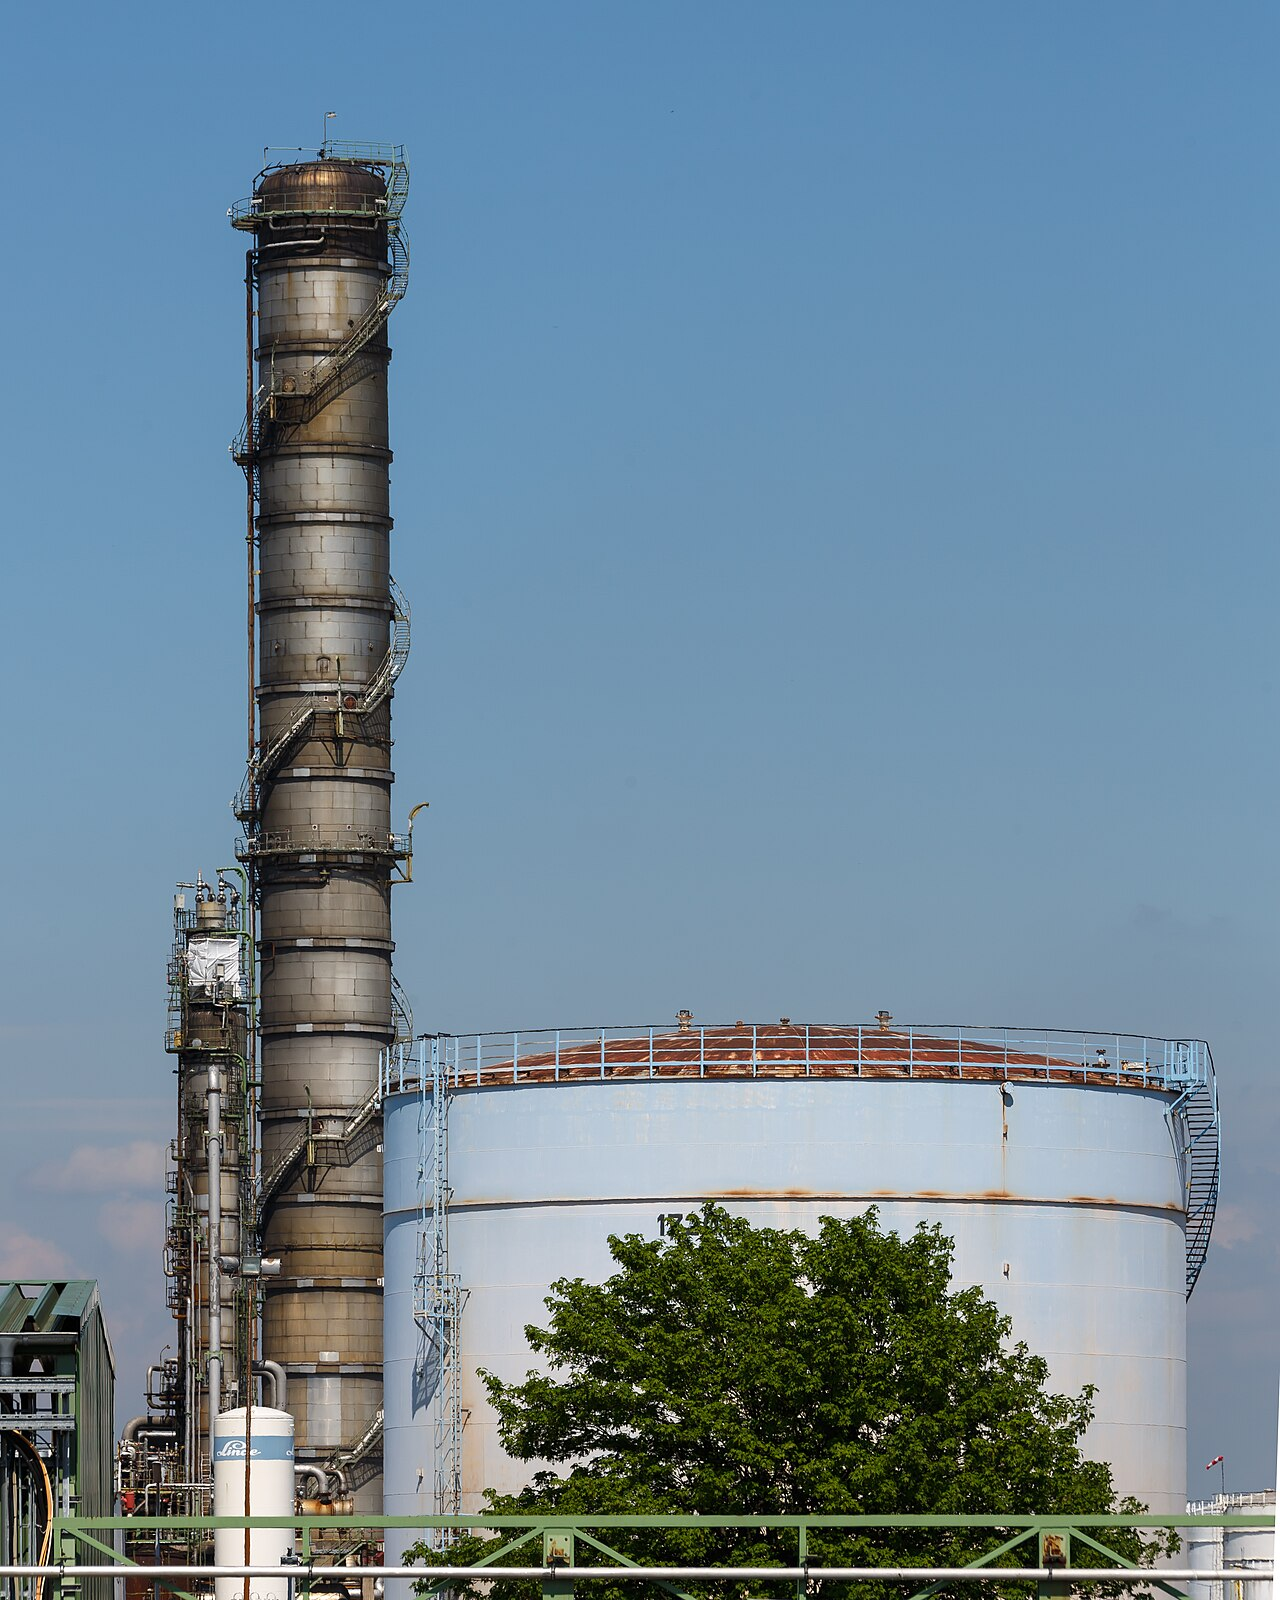
\includegraphics[width=\linewidth]{images/book3/refinery-column.jpg}
\end{minipage}

{\small 左：板式塔。液体流过每块塔板，经降液管流到下方的塔板；
蒸气向上穿过各块塔板，在液体中鼓泡。冷凝蒸气的一部分
作为回流返回塔内；塔底的再沸器提供蒸气。右：
科隆某炼油厂的精馏塔（2014 年），塔内有数十块塔板。（照片：
CEphoto，Uwe Aranas，CC BY-SA 3.0，
维基共享资源。）}
\end{omfigure}

\begin{proposition}[费恩斯克]\label{prop:b2:liquid-vapour-diagrams:fenske}
在全回流、相对挥发度 $\alpha$ 为常数时，
由塔底液体 $x_B$ 到馏出液
$x_D$ 所需的理论塔板数至少为
\[
  N_{\min} = \frac{1}{\ln\alpha}\,\ln\!\left[\frac{x_D}{1 - x_D}\cdot\frac{1 - x_B}{x_B}\right] .
\]
\end{proposition}

\begin{proof}
自下而上给塔板编号，再沸器为第 1 块板。全回流时，
第 $k + 1$ 块板上流下的液体，其组成
与离开第 $k$ 块板的蒸气相同：$x_{k+1} = y_k$。令 $r = x/(1 - x)$，则每块板给出
$r(y_k) = \alpha\,r(x_k)$，于是 $r(x_{k+1}) = \alpha\,r(x_k)$，经过 $N$ 块
板后冷凝蒸气满足 $r(x_D) = \alpha^N r(x_B)$。取对数，
便得 $N$。有限回流时，向下流的液体比上升的蒸气更贫，
每块板的增浓作用更弱，需要更多的塔板。
\end{proof}

在 $(x, y)$ 图上，同样的作图是夹在
平衡曲线与对角线 $y = x$ 之间的阶梯线，每一步
对应一块理论塔板。

\begin{omfigure}
\begin{tikzpicture}
\begin{axis}[width=0.55\linewidth, height=0.55\linewidth, xmin=0, xmax=1,
  ymin=0, ymax=1, axis x line=bottom, axis y line=left,
  xlabel={$x$（苯，液相）}, ylabel={$y$（苯，蒸气）},
  tick label style={font=\small}, label style={font=\small}]
\addplot[omThm, thick] table[x=x, y=y] {figdata/out/bachelor-2-liquid-vapour-f-eq.dat};
\addplot[black!50] coordinates {(0,0) (1,1)};
\addplot[omDef, thick] table[x=x, y=y] {figdata/out/bachelor-2-liquid-vapour-f.dat};
\draw[densely dotted] (axis cs:0.95,0) -- (axis cs:0.95,0.95);
\draw[densely dotted] (axis cs:0.05,0) -- (axis cs:0.05,0.05);
\node[font=\scriptsize, anchor=south east] at (axis cs:0.945,0.02) {$x_D$};
\node[font=\scriptsize, anchor=south west] at (axis cs:0.05,0.02) {$x_B$};
\end{axis}
\end{tikzpicture}

{\small 苯–甲苯体系在全回流下的塔板图，从馏出液组成
0.95 出发向下：每条水平线段从蒸气连到与之平衡的液体（即一块塔板），
每条竖直线段从该液体连到下方塔板的蒸气。
七步即可使液体组成降到 $x_B = 0.05$ 以下；
由费恩斯克公式得 6.5。}
% ledger: antoine:benzene.A, antoine:toluene.A (computed in figdata/bachelor-2/liquid-vapour.py)
\end{omfigure}

\begin{proposition}[精馏塔不能越过共沸物]\label{prop:b2:liquid-vapour-diagrams:azeotrope-limit}
对于含共沸物的混合物，若精馏塔的进料位于共沸组成的某一侧，
则至多能在一端得到共沸物，
在另一端得到该侧的纯组分。
\end{proposition}

\begin{proof}
在共沸点处，平衡曲线与对角线相交：$y = x$。在其附近，
阶梯的每一步都变得无穷小，因此有限块塔板
都无法到达它，也不能越过它。
\end{proof}

\begin{method}[预测分馏结果]\label{met:b2:liquid-vapour-diagrams:predict-distillation}
\begin{enumerate}
  \item 在等压相图上，找出进料可达到的最低沸点，即纯组分
        或正共沸物。它
        在塔顶馏出。
  \item 同侧的最高沸点（纯组分
        或负共沸物）留在釜中。
  \item 若存在共沸物，看进料位于它的哪一侧：只能得到
        该侧的纯组分。
  \item 求塔板数时，用费恩斯克公式或阶梯图，
        再为实际使用的有限回流增加塔板数。
\end{enumerate}
\end{method}

对于乙醇和水，进料组成低于 0.881 时，塔顶至多得到
共沸物，塔底得到水：没有任何精馏塔能得到无水乙醇。
除去最后百分之几的水，需要另一种方法——例如吸附水的分子筛，
或加入第三组分以破坏共沸物。

\begin{omfigure}
\begin{tikzpicture}[font=\small, scale=0.95, >={Stealth}]
  \pic[transform shape] at (0,0) {heatingmantle};
  \pic[transform shape] at (0,0) {rbflask={0.45}{orange!25}};
  \foreach \x/\y in {-0.35/0.25,0.05/0.18,0.35/0.3}
    \fill[black!55] (\x,\y) circle (0.06);
  % Vigreux column from the flask neck (0,3) to (0,6)
  \draw[om glass] (-0.22,3.0) -- (-0.22,6.0) (0.22,3.0) -- (0.22,6.0);
  \foreach \yy in {3.4,3.9,4.4,4.9,5.4} {
    \draw[om glass] (-0.22,\yy) -- (-0.06,\yy+0.18) -- (-0.22,\yy+0.3);
    \draw[om glass] (0.22,\yy+0.15) -- (0.06,\yy+0.33) -- (0.22,\yy+0.45);
  }
  \pic[transform shape] (s) at (0,6.0) {stillhead};
  \pic[transform shape] at ($(s-top)+(0,-0.75)$) {thermometer};
  \pic[transform shape, rotate=-20] (c) at (s-arm) {liebig={3.4}};
  % ground-glass joint between the head's side arm and the condenser
  \draw[om glass, fill=white, rotate around={-20:(s-arm)}] ($(s-arm)+(-0.12,-0.17)$) rectangle ($(s-arm)+(0.14,0.17)$);
  \coordinate (cend) at ($(s-arm)+(-20:3.4)$);
  \pic[transform shape] (a) at (cend) {adapter};
  \pic[transform shape] at ($(a-tip)+(0,-2.4)$) {erlenmeyer={0.22}{orange!12}};
  \draw[<-, omProp, thick] (-0.25,4.6) -- (-1.6,4.6) node[left, text=black,
    align=right] {维格勒分馏柱 \\ （凹痕增加接触点）};
  \draw[<-, omProp, thick] (0.12,6.72) -- (-1.4,7.4) node[left, text=black,
    align=right] {温度计球泡 \\ 与侧管平齐};
  \draw[<-, omProp, thick] (1.08,0.3) -- (2.3,-0.2) node[right, text=black]
    {加热套};
  \draw[<-, omProp, thick] ($(a-tip)+(0.75,-2.0)$) -- ++(1.0,0.2)
    node[right, text=black] {馏出液};
\end{tikzpicture}

{\small 实验室中的分馏。烧瓶与蒸馏头之间的维格勒分馏柱起到若干理论塔板的作用：
蒸气在其凹痕处凝结，并在上升途中再次蒸发。
只要仍有馏出液，蒸馏头处的温度
便保持在最易挥发组分的沸点，
此后才上升。}
\end{omfigure}

\begin{inthelab}[用分馏法分离两种液体]
烧瓶至多装入一半的液体，加入沸石，缓慢加热，
使冷凝蒸气形成的环缓慢上升通过分馏柱：加热过快
会使分馏柱失去塔板的作用。每隔几毫升记录一次蒸馏头温度，
温度开始上升时更换接收器（每个温度区间收集一份
\textit{馏分}），并在烧瓶蒸干之前
停止加热。
\end{inthelab}

\section{部分互溶与不互溶的液体}

\begin{definition}[互溶间隙]\label{def:b2:liquid-vapour-diagrams:miscibility-gap}
称\emph{互溶间隙}\index{互溶间隙}为两种液体在给定温度下分成两液层时
所对应的总组成范围，
每一液层都被另一组分饱和。
称\emph{非均相共沸物}\index{非均相共沸物}为这种两液层液体的
沸点：两液层与蒸气在固定温度下共存，
且蒸气组成固定。
\end{definition}

在非均相共沸点，两组分处于三相共存：在固定
压强下自由度为 $2 + 2 - 3 - 1 = 0$。温度保持
不变，与纯液体的沸点相同，只要两液层
仍然存在。

\begin{omfigure}
\begin{tikzpicture}[font=\small, x=6cm, y=0.08cm]
  \draw[->] (0,0) -- (1.05,0) node[right] {$x$};
  \draw[->] (0,0) -- (0,62) node[above] {$T$};
  \node[below] at (0,0) {2}; \node[below] at (1,0) {1};
  % boiling points: 2 at 50, 1 at 42; heteroazeotrope at 25 with layers 0.1 and 0.85, vapour 0.6
  \draw[omliquidus] (0,50) .. controls (0.04,38) and (0.08,30) .. (0.1,25);
  \draw[omliquidus] (1,42) .. controls (0.95,34) and (0.9,28) .. (0.85,25);
  \draw[omsolidus] (0,50) .. controls (0.25,46) and (0.5,35) .. (0.6,25);
  \draw[omsolidus] (1,42) .. controls (0.9,37) and (0.7,30) .. (0.6,25);
  \draw[thick] (0.1,25) -- (0.85,25);
  \draw[omliquidus] (0.1,25) -- (0.07,2);
  \draw[omliquidus] (0.85,25) -- (0.9,2);
  \fill (0.6,25) circle[radius=2pt];
  \node[font=\scriptsize] at (0.47,6) {两液层};
  \node[font=\scriptsize] at (0.5,55) {蒸气};
  \node[font=\scriptsize] at (0.035,12) {L$_2$};
  \node[font=\scriptsize] at (0.96,12) {L$_1$};
  \node[font=\scriptsize, align=center] at (0.3,33) {L$_2$ + V};
  \node[font=\scriptsize, anchor=west] at (1.06,36) {L$_1$ + V};
  \draw[thin] (1.06,36) -- (0.86,29.5);
  \node[font=\scriptsize, anchor=north] at (0.6,24) {非均相共沸物};
\end{tikzpicture}

{\small 两种部分互溶液体的等压相图示意图。非均相共沸温度以下，
液体分为两液层 L$_1$ 和
L$_2$，组成范围很宽（即互溶间隙）；沿水平线
两液层同时沸腾，生成组成固定的
蒸气（圆点处）。}
\end{omfigure}

\begin{definition}[水蒸气蒸馏]\label{def:b2:liquid-vapour-diagrams:steam-distillation}
称\emph{水蒸气蒸馏}\index{水蒸气蒸馏}为通过通入水蒸气
来蒸馏与水不互溶的液体的过程：混合物
的沸点低于两种液体各自的沸点，馏出液分为
两层。
\end{definition}

水蒸气蒸馏与第 1 册中的水蒸气蒸馏
只在水的引入方式上不同：通入物料中的是水蒸气，
而非将物料在水中煮沸。热力学原理相同。

\begin{proposition}[两种不互溶液体的沸腾]\label{prop:b2:liquid-vapour-diagrams:steam}
两种互不相溶的液体接触时，在两者蒸气压之和
等于外压的温度下沸腾，即 $p_1^*(T) + p_2^*(T) =
p$，且低于两者各自的沸点。馏出液中两种液体的
质量比为
\[
  \frac{m_1}{m_2} = \frac{p_1^*\,M_1}{p_2^*\,M_2} .
\]
\end{proposition}

\begin{proof}
每种纯液体都产生自身的蒸气压，与另一组分的
量无关：两液层上方的总压为 $p_1^* + p_2^*$，
在某一温度下达到 $p$，此时每个 $p_i^*$ 均小于 $p$。在
蒸气中，两组分的物质的量与其分压成正比，$n_1/n_2 =
p_1^*/p_2^*$；乘以 $M_1/M_2$ 即可。
\end{proof}

\begin{omfigure}
\begin{tikzpicture}
\begin{axis}[width=0.6\linewidth, height=5.5cm, xmin=70, xmax=100, ymin=0, ymax=1.6,
  axis x line=bottom, axis y line=left, xlabel={$T$ (\unit{\degreeCelsius})},
  ylabel={$p$ (\unit{bar})}, tick label style={font=\small},
  label style={font=\small}, clip=false]
\addplot[omProp, thick] table[x=t, y=ptol] {figdata/out/bachelor-2-liquid-vapour-e.dat};
\addplot[omDef, thick] table[x=t, y=pwat] {figdata/out/bachelor-2-liquid-vapour-e.dat};
\addplot[black, very thick] table[x=t, y=psum] {figdata/out/bachelor-2-liquid-vapour-e.dat};
\draw[densely dashed] (axis cs:70,1.013) -- (axis cs:100,1.013) node[right, font=\scriptsize] {\qty{1.013}{bar}};
\draw[densely dotted] (axis cs:84.3,0) -- (axis cs:84.3,1.013);
\node[font=\scriptsize, anchor=south east] at (axis cs:84.3,1.05) {\qty{84.3}{\degreeCelsius}};
\node[font=\scriptsize, anchor=west] at (axis cs:96,1.45) {总和};
\node[font=\scriptsize, omDef, anchor=south] at (axis cs:77,0.46) {水};
\node[font=\scriptsize, omProp, anchor=north west] at (axis cs:88,0.5) {甲苯};
\end{axis}
\end{tikzpicture}

{\small 甲苯与水不互溶：各液体的蒸气压及其
之和。两层液体在 \qty{84.3}{\degreeCelsius} 下共同沸腾，
低于水（\qty{100}{\degreeCelsius}）与甲苯（\qty{110.6}{\degreeCelsius}）的沸点；
馏出液中每克水携带 4.1 g 甲苯。}
% ledger: antoine:toluene.A, antoine:water.A, aw:C, aw:H, aw:O (computed in figdata/bachelor-2/liquid-vapour.py)
\end{omfigure}

植物精油中沉重、不稳定的分子以此法蒸馏，
在略低于 \qty{100}{\degreeCelsius} 下进行，远低于其自身沸点，
分解很少；代价是馏出液中大部分为水。

\section{练习}

\begin{exercise}[$\star$]\label{exo:b2:liquid-vapour-diagrams:1}
在苯–甲苯等压相图上，读出两种纯液体的沸点、
组成为 0.2 的液体的泡点，以及
其初始蒸气的组成。
\end{exercise}

\begin{exercise}[$\star$]\label{exo:b2:liquid-vapour-diagrams:2}
在 \qty{80}{\degreeCelsius} 时，苯与甲苯的蒸气压分别为
\qty{1.010}{bar} 和 \qty{0.388}{bar}。对等摩尔液体，求
其开始沸腾时的压强，以及蒸气的组成。
\end{exercise}

\begin{exercise}[$\star$]\label{exo:b2:liquid-vapour-diagrams:3}
\qty{10}{mol} 总组成为 0.30 的混合物处于某一温度，
此时液相组成为 0.20，气相组成为 0.45。求
各相的物质的量。
\end{exercise}

\begin{exercise}[$\star$]\label{exo:b2:liquid-vapour-diagrams:4}
求苯–甲苯混合物的自由度：(a) 全为液体；(b)
沸腾中；(c) 恒压下处于共沸点（对存在共沸物的体系）。
\end{exercise}

\begin{exercise}[$\star\star$]\label{exo:b2:liquid-vapour-diagrams:5}
用试差法求组成为 0.30 的苯–甲苯蒸气在
\qty{1.013}{bar} 下的露点，用 $p^*_{\text{苯}}$ 和 $p^*_{\text{甲苯}}$
（\unit{bar}）：在 \qty{100}{\degreeCelsius} 时为 1.80 和 0.742；
在 \qty{105}{\degreeCelsius} 时为 2.057 和 0.861。给出第一滴液体的组成。
\end{exercise}

\begin{exercise}[$\star\star$]\label{exo:b2:liquid-vapour-diagrams:6}
等摩尔的苯–甲苯混合物作简单蒸馏（无精馏塔）。
求首批馏出液的组成，以及馏出液的温度与组成
随蒸馏进行如何变化，
并说明分离效果为何较差。
\end{exercise}

\begin{exercise}[$\star\star$]\label{exo:b2:liquid-vapour-diagrams:7}
乙醇摩尔分数为 0.05 的葡萄酒，用
效率很高的精馏塔进行分馏。塔顶馏出什么，塔釜留下什么？
对摩尔分数为 0.95 的混合物，同样回答上述问题。
\end{exercise}

\begin{exercise}[$\star\star$]\label{exo:b2:liquid-vapour-diagrams:8}
植物精油中的一种组分（摩尔质量 \qty{136}{g/mol}）
在 \qty{97}{\degreeCelsius} 附近的蒸气压为 \qty{0.10}{bar}，此时水的蒸气压为
\qty{0.91}{bar}（习题数据）。求在 \qty{1.013}{bar} 下
水蒸气蒸馏进行的温度，以及
每克水可收集精油多少克。
\end{exercise}

\begin{exercise}[$\star\star$]\label{exo:b2:liquid-vapour-diagrams:9}
在部分互溶液体的示意相图上，描述总组成为 0.4 的两层混合物
自室温加热至全部为蒸气时所发生的变化：
所经历的相态、温度，以及
首个蒸气的组成。
\end{exercise}

\begin{exercise}[$\star\star\star$]\label{exo:b2:liquid-vapour-diagrams:10}
取 $\alpha = 2.47$，求馏出液组成为 0.99、塔釜为 0.01 时
所需理论塔板数的最小值；与馏出液 0.95、塔釜 0.05 所需的 6.5 块比较，
并评论提纯的代价。
\end{exercise}

\begin{exercise}[$\star\star\star$]\label{exo:b2:liquid-vapour-diagrams:11}
由苯–甲苯等压相图及安托万方程，
说明如何得到 \qty{80}{\degreeCelsius} 下的等温相图，
以及其中液相区为何位于上方。
\end{exercise}

\begin{exercise}[$\star\star\star$]\label{exo:b2:liquid-vapour-diagrams:12}
从关系式 $d\ln p = (y - x)\,dy/[y(1 - y)]$ 出发，证明在恒温下，
凡蒸气中组分 1 的含量高于液相处，总压强随 $x$ 增大，
并由此推出理想混合物不存在
共沸物。
\end{exercise}

\section{问题：苯与甲苯的精馏塔}

\begin{problem}[{周末问题——由安托万方程求得苯与
甲苯的等压相图，闪蒸与杠杆规则，
全回流时精馏塔的最少塔板数，以及
共沸物所设定的极限}]
\label{pb:b2:liquid-vapour-diagrams:1}
数据：安托万方程 $\log_{10}(p^*/\unit{bar}) = A - B/(T + C)$，其中 $T$ 以
开尔文计：苯 $A = 4.01814$，$B = \qty{1203.835}{K}$，$C =
\qty{-53.226}{K}$；甲苯 $A = 4.07827$，$B = \qty{1343.943}{K}$，$C =
\qty{-53.773}{K}$。压强为 \qty{1.013}{bar}；苯与甲苯组成理想
混合物。乙醇–水共沸物中乙醇的质量分数为 95~\%。
% ledger: antoine:benzene.A, antoine:benzene.B, antoine:benzene.C, antoine:toluene.A, antoine:toluene.B, antoine:toluene.C, azeo:ethanol-water.w

\medskip
\noindent\textbf{第一部分——相图。}
\begin{enumerate}
  \item 求苯与甲苯在 \qty{1.013}{bar} 下的沸点。
  \item 求 \qty{90}{\degreeCelsius} 下的 $p_1^*$ 与 $p_2^*$。
  \item 推出平衡时液相与气相在
        \qty{90}{\degreeCelsius} 下的组成。
  \item 在 \qty{100}{\degreeCelsius} 下同样求解（$p_1^* = \qty{1.800}{bar}$，$p_2^* =
        \qty{0.742}{bar}$）。
  \item 由以上四点及两种纯液体画出等压相图。
  \item 用试差法求等摩尔液体的泡点，精确到
        \qty{0.5}{\degreeCelsius}，试差范围在 \qty{90}{\degreeCelsius} 与
        \qty{95}{\degreeCelsius} 之间。
  \item 求沸腾混合物的自由度，并说明它
        对相图意味着什么。
\end{enumerate}

\medskip
\noindent\textbf{第二部分——闪蒸。}
\begin{enumerate}[resume]
  \item 将等摩尔进料加热至 \qty{95}{\degreeCelsius}（$p_1^* =
        \qty{1.569}{bar}$，$p_2^* = \qty{0.636}{bar}$）。求 $x$ 与 $y$。
  \item 对于 \qty{100}{mol} 进料，求液相与气相的物质的量。
  \item 求每一相中苯的物质的量，并检验物料平衡。
  \item 气相中回收的苯占总苯量的几分之几？
  \item 若闪蒸在 \qty{100}{\degreeCelsius} 下进行，会发生什么？
  \item 进料在何温度下恰好全部汽化？
\end{enumerate}

\medskip
\noindent\textbf{第三部分——精馏塔。}
\begin{enumerate}[resume]
  \item 定义相对挥发度 $\alpha$，并求其在苯的
        沸点处的值。
  \item 求其在甲苯沸点处的值。
  \item 取几何平均值作为整个塔的值。
  \item 证明在理论塔板上 $y/(1 - y) = \alpha\,x/(1 - x)$。
  \item 解释为何在全回流时，进入某塔板的液体
        与其下方塔板离开的蒸气组成相同。
  \item 推导芬斯克公式。
  \item 求馏出液为 0.95、釜液为 0.05 时所需
        理论塔板的最少数目。
  \item 为何实际精馏塔所需塔板数比这更多？
  \item 在本章的阶梯图上数出台阶数，并进行比较。
\end{enumerate}

\medskip
\noindent\textbf{第四部分——共沸物。}
\begin{enumerate}[resume]
  \item 求乙醇–水共沸物中乙醇的摩尔分数。
  \item 乙醇含量为 0.10 的进料进入一座有五十块塔板的塔，
        塔顶与塔底各离开什么？
  \item 写出将苯与甲苯分离为 95~\% 产品所需的
        理论塔板的最少数目。
\end{enumerate}
\end{problem}
